
\begin{frame}[c]
 \frametitle{Case study}
 

\tval{Lambda phage} : ($4$  components and $11$  interactions); 

\tval{EGF/TNF} : ($28$  components and $55$  interactions); 

\tval{t\_helper differentiation}: ($101$  components and $381$  interactions).

\begin{center}
  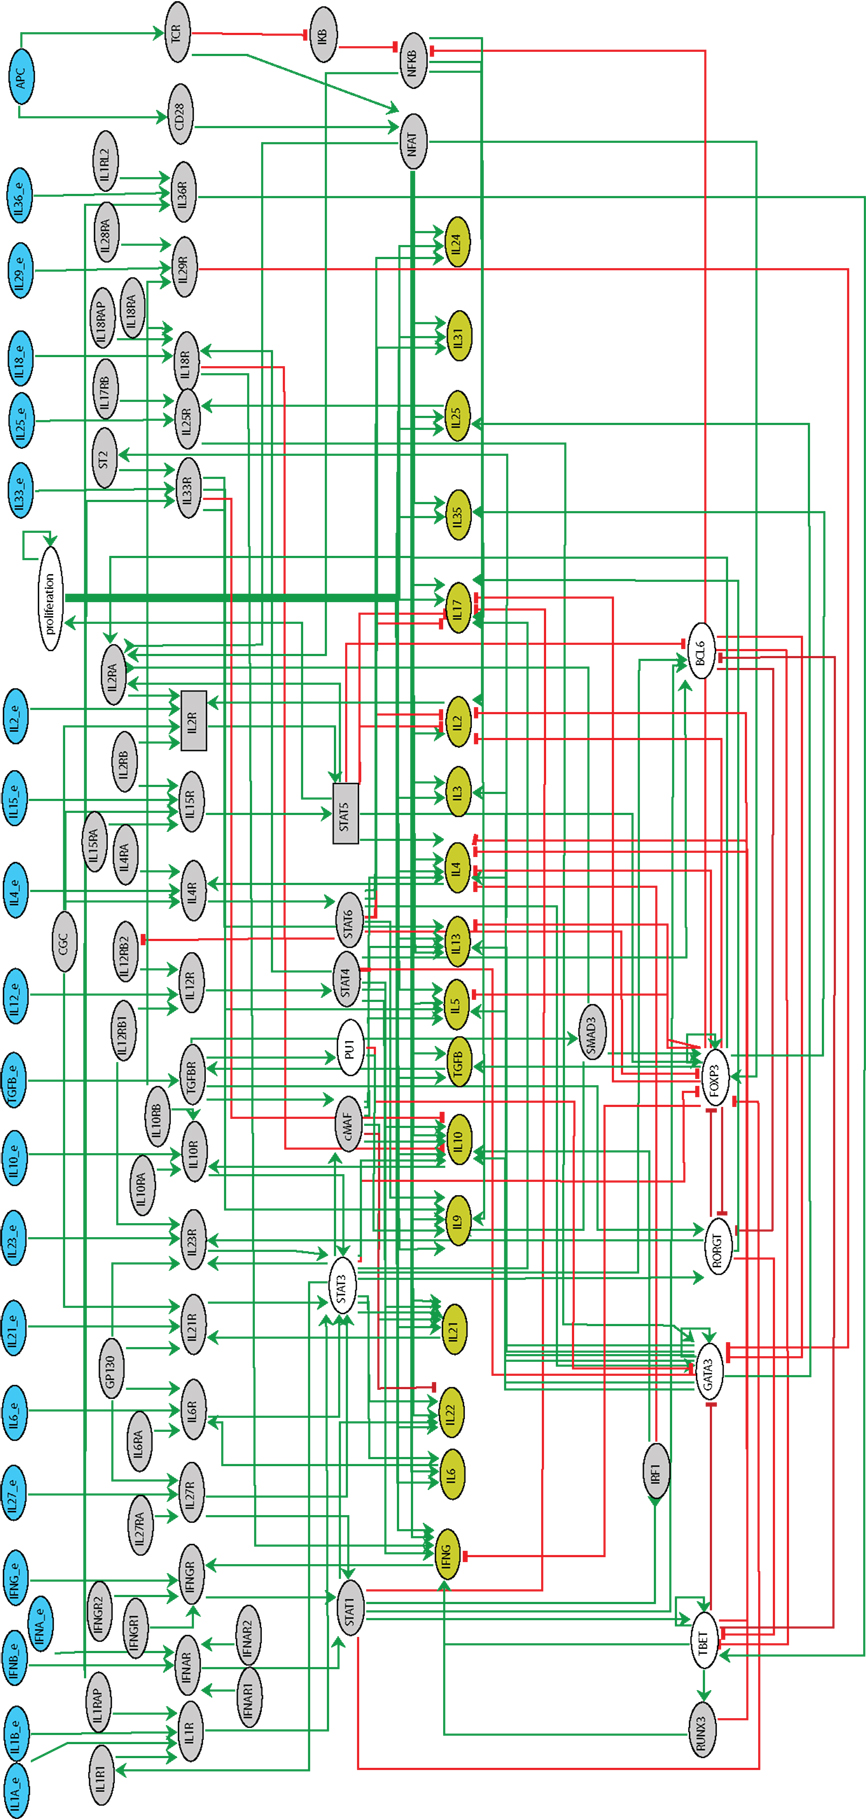
\includegraphics[scale=0.18,angle=-90]{images/th_differentiation.jpg}
\end{center}
\begin{center}
 {\tiny \color{darkgreen} [\citeatfb]}
\end{center}
\end{frame}



%mettre le tableau
\begin{frame}[c]
 \frametitle{Results of identification of bifurcations}
 

%mettre le tableau
\begin{table}[bt]
\renewcommand{\arraystretch}{1.3}

\centering
%table of result
\scalebox{0.8}{
\setlength{\tabcolsep}{2mm}
\begin{tabular}{|c|c||c|r||c|r||c|r|}
\hline
\multirow{2}{*}{Automata Network} 
& \multirow{2}{*}{Goal}
& \multicolumn{2}{c||}{M-C (NuSMV)}
& \multicolumn{2}{c||}{with \iIIIa}
& \multicolumn{2}{c|}{with \iIIIb}
\\
\cline{3-8}
&&$\card{t_b}$&Time&$\card{t_b}$&Time&$\card{t_b}$&Time
\\\hline

Lambda phage &  $\mathrm{CI}_2$ & $10$ & $0.1s$ & $6$ & $0.1s$ & $0$ & $0.2s$ 	
\\
$\card\anN=4\quad\card\anT=11$ &$\mathrm{Cro}_2$ & $3$ & $0.1s$ & $3$ & $0.1s$ & $2$ & $0.3s$ 	
\\ \hline 

EGF/TNF       & $\mathrm{NFkB}_0$ & $5$ & $0.2s$ & $4$ & $0.1s$ & $2$ & $0.1s$ 
\\

$\card\anN=28\quad\card\anT=55$ & $\mathrm{IKB}_1$ & $5$ & $0.2s$ & $3$ & $0.1s$ & $2$ & $0.1s$ 

\\ \hline

Th\_th17 & $\mathrm{RORGT}_1$ & $18$ & $48s$ & $9$ & $23s$ & $8$ & $26s$  
\\
$\card\anN=101\quad\card\anT=381$ & $\mathrm{BCL6}_1$ &$7$ & $26s$ &$5$ & $23s$ & $4$ & $24s$ 

\\ \hline

Th\_HTG & $\mathrm{BCL6}_1$ & \multicolumn{2}{c||}{\multirow{2}{*}{out-of-time}} & \multicolumn{2}{c||}{\multirow{2}{*}{out-of-time}} & $6$ & $61s$ 

\\

$\card\anN=101\quad\card\anT=381$ & $\mathrm{GATA3}_1$ &  \multicolumn{2}{c||}{} &\multicolumn{2}{c||}{}  & $7$ & $34s$ 

\\ \hline



\end{tabular}
}
\end{table}
\begin{center} Implemented in ASP (Answer Set Programming) and solve with clingo 4.5.4.\end{center}
\end{frame}

\begin{frame}
%mettre cette slide un peu avant la conclusion
\frametitle{Automata Network modelling of Biological Networks}
\textbf{Transition-centered specification}
\begin{itemize}
\item ...in opposition to function-centered of Boolean/Thomas networks
\item explicit context/ \tval{causality of state changes}
\item closely related to (safe) Petri nets
\item step semantics (purely async, purely sync, mixed)
\end{itemize}
\textbf{Modelling}
\begin{itemize}
\item any Boolean/Thomas networks can be encoded;
\item in case of logical rules uncertainty: \tval{model the union} of Boolean/Thomas networks (over-approximation of behaviours)
%\item encoding of \tval{SBGN Process Description} models
\end{itemize}
\end{frame}
